\chapter{Ausblick}
\label{ch:Ausblick}

An dieser Stelle möchten wir einen Ausblick geben, wie der von uns entwickelte Gestikulaser  weiterentwickelt wird. \\
Hier wäre zunächst einmal eine Verfeinerung der aktuell durchführbaren Gestenerkennung denkbar, die nicht nur die Stellung der Hand, sondern auch die Krümmung der einzelnen Finger berücksichtigt. Zu diesem Zweck wurde bereits ein Prototyp für einen Sensorhandschuh entwickelt. 
\begin{figure}[H]
	\centering
	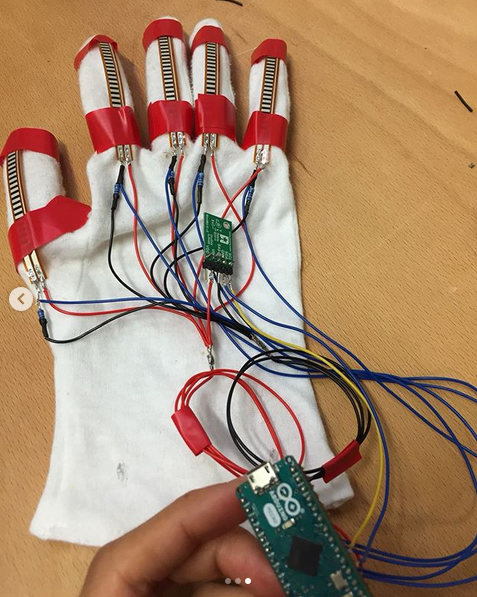
\includegraphics[scale=0.75]{../figures/Sensorhandschuh}
	\caption{Aktueller Prototyp des Sensorhandschuhs. Es sind Biegesensoren für alle Finger, ein Gyroskop und ein Beschleunigungssensor im Einsatz. Bei der  
	Verarbeitung der Sensordaten kommt ein Arduino Micro zum Einsatz.}
	\label{fig:Sensorhandschuh}
\end{figure}
\noindent
Dieser könnte während der Trainingsphase vom Nutzer dazu verwendet werden, feinere Gesten aufzunehmen, wobei neben den von den Detektormodulen detektierten Photoströmen zusätzlich die Daten der auf dem Sensorhandschuh befindlichen Module gespeichert werden. Aktuell kommen hier Biegesensoren für jeden Finger, sowie ein Gyroskop und ein Beschleunigungssensor zum Einsatz. Diese verfeinerten Gestendaten stellen nun natürlich eine neue Herausforderung an das Modell, das zur Auswertung der Photoströme im Live-Betrieb eingesetzt wird: Statt wie vorher den eingehenden Photoströmen nur das Klassenlabel einer Geste zuzuordnen, muss es nun in der Lage sein, auf Basis der gemessenen Photoströme die wahrscheinliche Lage der Hand, sowie die Krümmung der Finger vorauszusagen. Dieses Problem ist mathematisch deutlich schwieriger zu lösen, was nicht zuletzt an der deutlich höheren Anzahl an Parametern liegt, die bestimmt werden müssen, um eine ausreichende Aussagekraft zu gewährleisten. Aufgrund der höheren Anzahl an Parametern werden zudem auch mehr Daten benötigt, um das Modell zu trainieren. \\
Ebenfalls denkbar wäre eine Erweiterung auf dynamische Gesten, bei denen der Nutzer die Hand bewegt. In diesem Fall müssen die Daten der Photodioden im Live-Betrieb in Form Zeitreihe aufgenommen werden und das neuronale Netzmodell muss diese Zeitreihe mit einer Geste verknüpfen. Auch hier ergibt sich ein mathematisch deutlich komplexeres Problem, das ein aufwändigeres Training und viele Trainingsdaten erfordert. Die Erweiterung um dynamische Gesten könnte ebenfalls mit der Verwendung des Sensorhandschuhs kombiniert werden.

